\chapter{Data Link Layer}\label{ch:ch3label}

The data link layer aims to perform reliable node-to-node data delivery. We created a class called {\tt MAC} to handle this work. When the {\tt MAC} is started, it spawn a standalone receiving thread so that it works in full-duplex mode. This class can be used with python's context manager.

\section{Framing}

    \subsection{Structure}
        \subparagraph{}
        The general structure of the frames is shown below. The {\tt DST} and {\tt SRC} field are the destination and source MAC address. {\tt TYPE} is the type of the frame. {\tt FRAME\_ID} is the identity of the frame, which is unique for all frames execpt {\tt ACK} and {\tt PONG} types, and this will be explained in the next section. The {\tt PAYLOAD} can have a variable length from 0 to $(\text{MTU} - \text{MAC\_header})$, set by the user. When a frame is being transmitted, the MAC will encapsulate the essential information in this form.

        $$|DST (1B)|SRC(1B)|TYPE(1B)|FRAME\_ID(2B)|PAYLOAD(var)|$$

    \subsection{Types of Frames\textbf{}}
        \subparagraph{}
        There are five types of frames in our MAC: \texttt{START},\texttt{DATA},\texttt{ACK},\texttt{PING},\texttt{PONG}.
        
        \subsubsection{\texttt{START}}
            The \texttt{START} frame indicates the start of a sequence of frames, as a packet in the upper layer. The \texttt{TYPE} field has value 0. This packet has one byte in the \texttt{PAYLOAD} field, representing the \texttt{frame\_cnt}. The following \texttt{frame\_cnt} \texttt{DATA} frames are collected into one packet.
            
        \subsubsection{\texttt{DATA}}
            This type of frame contains the real data of the upper layer. The \texttt{TYPE} field has value 1. This \texttt{PAYLOAD} field is the data, and its length is given by the physical layer. The maximum length is usually $(\text{MTU} - \text{MAC\_header})$.

        \subsubsection{\texttt{ACK}}
            This frame is to acknowledge the sender that the previously transmitted frame has been correctly received. The \texttt{TYPE} field has value 2. These frames are transmitted whenever a \texttt{START} frame or a \texttt{DATA} frame has been received. One thing special about this kind of frame is that the \texttt{FRAME\_ID} field has the same value of the received \texttt{START} or \texttt{DATA} frame. This frame has no \texttt{PAYLOAD} field.

            There is something we would like to complain about. \texttt{ACK} is only needed in 802.11 MAC, which is CSMA/CA, but not in Ethernet MAC (CSMA).

        \subsubsection{\texttt{PING}}
            This frame is to do the ping test between MACs of two computers. The \texttt{TYPE} field has value 3. When a \texttt{PING} has been received, the receiver should reply a \texttt{PONG} frame with the same \texttt{FRAME\_ID}. This packet has no \texttt{PAYLOAD} field.

            There is something we would like to complain about. Real MAC does not have ping requests. This should work in the upper layer, just as the ICMP Echo Request/Reply.
        
        \subsubsection{\texttt{PONG}}
            This frame gives reply to the previous \texttt{PING} packet.  The \texttt{TYPE} field has value 4. The \texttt{FRAME\_ID} has the same value of the \texttt{PING} frame received.

    \subsection{Splitting Frames}
        \subparagraph{}
        Though splitting packet into frames should have been done in the upper layer, we had to do it in project 2 before we created the network layer in project 3. This the reason why we have \texttt{START} and \texttt{DATA} type and also require a MTU in our design, and the legacy code is left without modification since it is robust and provides a great functionality.
        \subparagraph{}
        When our MAC get a request to send a packet to the peer, the MAC requests a consecutive $m+1$ number of \texttt{FRAME\_ID}s. 1 is for a \texttt{START} frame and the $m$ is for $m=\lceil \text{packet\_length} / (\text{MTU} - \text{MAC\_header})  \rceil$ \texttt{DATA} frames. The $m$ frames are then filled with the slices of separated data.

    \subsection{Frame Length}
        \subparagraph{}
        The maximum \texttt{DATA} frame length is decided by $(\text{MTU} - \text{MAC\_header})$, as mentioned above. The maximum value of MTU is decided by the physical layer, which has 2 bytes for the \texttt{LENGTH} field. Therefore, the maximum length of one frame is $2^{16}=64KB$, which is, incidentally, the same size as a single TCP packet. Since the \texttt{START} frame has one byte for \texttt{FRAME\_CNT}, the maximum packet length we support is $64KB \times 256=16MB$. This gives us great flexibility and scalability. By far, we set a relatively small MTU of 1500B by default so that the transmission of one frame won't block the transmission of other frames forever.

\section{Receiving}
    \subparagraph{}
    Receiving thread is a standalone loop thread that always waits the physical layer to get a new frame. When the network is free, this thread is blocked by the physical layer queue. Aside from this, the receiver thread also needs to collect the consecutive \texttt{DATA} frames to recover a packet in the upper layer.

    \subsection{State Machine}
        \subparagraph{}
        To support the collection of the consecutive {\tt DATA} frames, we used a FSM to handle this job.
        
        {\hspace{4em}
        \begin{tikzpicture}[shorten >=1pt,node distance=6cm,on grid,auto]
            \node[state] (q_0)   {\makecell{Frame\\Detection}};
            \node[state] (q_1) [right=of q_0] {\makecell{Collect\\frames}};
            \path[-|>]
            (q_0) edge [bend left] node  {\makecell{Get START frame\\and FRAME\_CNT}} (q_1)
            (q_1) edge [bend left] node  {All frames collected} (q_0)
                edge [loop below] node {\makecell{Collect one DATA frame\\(need FRAME\_CNT times)}} ()
            ;
        \end{tikzpicture}
        }

        \subparagraph{}
        After rebuilding a full packet, the packet is put into the data queue within the MAC object. The packet can then be retrieved back by invoking {\tt recv} function. This function is just a simple call transfer to {\tt Queue.get}. The {\tt recv} function also supports a timeout so that the function can become non-blocking.

    \subsection{Limitation}\label{sec:lim}
    
        \subparagraph{}
        According to the state machine we show above, we now only support to collect one packet at a time. When the state machine start to collect \texttt{DATA} frames according to the last \texttt{START} frame, a new \texttt{START} frame will be \texttt{ACK}ed as if the \texttt{ACK} frame was lost or timed out. By far, the state machine cannot handle two sequence of frames at the same time. This means that we need to ensure the synchronization of sending so that the frames of two packets does not interleave with each other.
        \subparagraph{}
        This problem is discovered when we were writing the tunnel in project 4. For more details, refer to section \ref{sec:ftpsynch}.

\section{Sending}
    \subparagraph{}
    The sending function is a blocking function that can be invoked in any thread. In most cases, this is only invoked by the network layer, but it can still work if the users wants to control the MAC on their own.

    \subsection{Stop and wait}
        \subparagraph{}
        Project 2 requires us to implement a stop-and-wait protocol for sending frames, and the following figure is the state machine for this protocol. This is the default strategy for sending {\tt PING} and {\tt START}.

        \begin{figure}[!h]
	        \centering
	        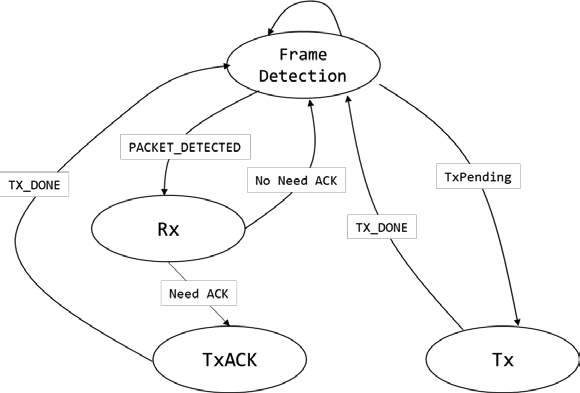
\includegraphics[width=0.5\linewidth]{sections/a.png}
	    \caption{Stop-and-wait state machine}
        \end{figure}
        
        When the MAC gets a frame detected by the physical layer, it first checks if the {\tt DST} field correctly matches the MAC address of itself or if it is a broadcast frame. We denote {\tt 0xff} as the broadcast frame MAC address.

    \subsection{Simple Sliding Window}
        To improve throughput, we added a simple sliding window with fixed window size. Instead of send one frame and wait for one ACK, we send window size of frames in a role and wait for all the ACKs. There could have been one improvement for future work to use the accumulative ACK just like the TCP transmission algorithm. After waiting for a certain amount of time set by the user, the sender checks if there is any frame still not ACKed, and then retransmit them in the next loop. This is the default strategy for sending {\tt DATA} frames.

    \subsection{LT Fountain Encoding}
        When we were handling the network with jamming, we tried to use LT fountain encoding to replace the sliding window algorithm, so that the receiver would not stuck on one frame for a long time. In this strategy, we only send one ACK when the receiver has enough data to recover the whole packet. The sender keeps sending newly generated frame yielded by the encoder and waits for the single ACK. This strategy is disabled by default, but users can enable it on their own.

    \subsection{Priority Queuing}
        To improve the latency of the control frames, including {\tt ACK}, {\tt PING}, {\tt PONG}, we give them a higher priority. The data frames, including {\tt START} and {\tt DATA} has lower priorities. We used the {\tt PriorityQueue} from python library and added the priority tag for each frame to be sent. This ensures that all the control frames, which aims for short latency, to be sent instantly without queuing with the data frames.

    \subsection{Multi-level Random Queue}
        Though priority queue can improve the latency for small control frames, it may block data frame forever when the amount of control frames is too overwhelming. In this case, the throughput of data frames will show great degradation. Thus, we added some pseudo-randomization to ensure the two kinds of frames are transmitted fairly. The chance for transmitting data frames is 25\% and the chance for transmitting control frames is 75\%. Since data frames have relatively large size and control frames have relatively small size, it is acceptable to have a 1:3 chance proportion. This strategy is also disabled by default but users can enable it on their own.

    \subsection{Synchronization}
        As stated in section \ref{sec:lim}, we added a global lock in the MAC object. In the prologue of the data sending function, it acquires the lock. In the epilogue of the data sending function, it releases the lock. The critical section code ensures that no {\tt Exception} would be raised from inside so the lock resource is ensured to be well-managed. For functions that send other frames, including {\tt ACK}, {\tt PING} and {\tt PONG}, we do not need to add the lock, because the frames are queued in the physical layer using python's Queue, which is already atomic by nature.

\section{Carrier Sense Multiple Access}
\subparagraph{}
Carrier Sense Multiple Access(CSMA) request listening the transmission media before send data. Notice in our design of the physical layer, not only we calculate the dot result of the received signal and the template one, but also the power of the former one. Then we can divided the status of the transmission media into three cases:
\begin{itemize}
    \item idle: The power is low
    \item transferring: The power is high, the dot is large
    \item jamming/noise: The power is high, the dot is low
\end{itemize}
Only in the first case we can start a new process of transmission. In the last case that the channel is busy while the content do not match the sending ones, we can judge that there are other nodes using this channel or terrible interfere occurs and we then block the sending thread. After the channel get idle, we execute the back-off strategy and resume the blocked thread(if exists) then the sending function is available again.